\documentclass[12pt,afrikaans, english,letterpaper,oneside,
openany]{memoir}

%==== Graphics and Color ============================================
  \usepackage{graphicx}%........................... Graphicx loaded in usthesis
\usepackage{color}%.............................. Color setup
\usepackage{eso-pic}%............................ Shipout commands for watermark
\newcommand*{\WaterMark}[2][0.15\paperwidth]{%
  \AddToShipoutPicture*{\AtTextCenter{%
    \parbox[t]{0pt}{\makebox[0pt][c]{%
      \includegraphics[width=#1]{#2}}}}}}
                         
                         \usepackage[masters-t, goldenblock,]{usthesis} % option to replace masters-t with PhD 
                                                                         \usepackage{lmodern}
                                                                         \usepackage{amssymb,amsmath}
                       \usepackage{ifxetex,ifluatex}
                       \usepackage{textcomp}
                       \usepackage{bm}
                       \usepackage{fixltx2e} % provides \textsubscript
                       \ifnum 0\ifxetex 1\fi\ifluatex 1\fi=0 % if pdftex
                       \usepackage[T1]{fontenc}
                       \usepackage[utf8]{inputenc}
                                                \else % if luatex or xelatex
                                                \usepackage{unicode-math}
                                                \defaultfontfeatures{Ligatures=TeX,Scale=MatchLowercase}
                                                                                                                                                                                                      \fi
                       % use upquote if available, for straight quotes in verbatim environments
                       \IfFileExists{upquote.sty}{\usepackage{upquote}}{}
                       % use microtype if available
                       \IfFileExists{microtype.sty}{%
                         \usepackage[]{microtype}
                         \UseMicrotypeSet[protrusion]{basicmath} % disable protrusion for tt fonts
                       }{}
                       \PassOptionsToPackage{hyphens}{url} % url is loaded by hyperref
                                                \usepackage[unicode=true]{hyperref}
                       \usepackage[capitalize]{cleveref} % delete if not working
                                                \hypersetup{
                                                        pdftitle={An Econometric Analysis of the Illicit South African Tobacco Market},
                                                                                           pdfauthor={Cassandra Pengelly},
                                                                                                                                        pdfborder={0 0 0},
                                                                            breaklinks=true}
                       \urlstyle{same}  % don't use monospace font for urls
\ifnum 0\ifxetex 1\fi\ifluatex 1\fi=0 % if pdftex
  \usepackage[shorthands=off,main=]{babel}
\else
  \usepackage{polyglossia}
  \setmainlanguage[]{}
\fi
\usepackage{usnomencl}
\usepackage{acronym}
%\usepackage{natbib}
%\bibliographystyle{plainnat}
\usepackage{usbib}%.............................. Bibliography    (in usthesis pack)
    \bibliographystyle{usmeg-a}
    \renewcommand\bibfont{\small}

    %% For usmeg-a, the bib is a list of references. If you
    %% are using usmeg-n comment out the following lines
    \addto{\captionsafrikaans}{\renewcommand{\bibname}{Lys van Verwysings}}
    \addto{\captionsenglish}{\renewcommand{\bibname}{List of References}}
\IfFileExists{parskip.sty}{%
\usepackage{parskip}
}{% else
\setlength{\parindent}{0pt}
\setlength{\parskip}{6pt plus 2pt minus 1pt}
}
\setlength{\emergencystretch}{3em}  % prevent overfull lines
\providecommand{\tightlist}{%
  \setlength{\itemsep}{0pt}\setlength{\parskip}{0pt}}
\setcounter{secnumdepth}{5}
% Redefines (sub)paragraphs to behave more like sections
\ifx\paragraph\undefined\else
\let\oldparagraph\paragraph
\renewcommand{\paragraph}[1]{\oldparagraph{#1}\mbox{}}
\fi
\ifx\subparagraph\undefined\else
\let\oldsubparagraph\subparagraph
\renewcommand{\subparagraph}[1]{\oldsubparagraph{#1}\mbox{}}
\fi

% set default figure placement to htbp
\makeatletter
\def\fps@figure{htbp}
\makeatother

\usepackage{subfig}
\usepackage{array}
\usepackage{caption}
\usepackage{graphicx}
\usepackage{siunitx}
\usepackage[normalem]{ulem}
\usepackage{colortbl}
\usepackage{multirow}
\usepackage{hhline}
\usepackage{calc}
\usepackage{tabularx}
\usepackage{threeparttable}
\usepackage{wrapfig}
\usepackage{adjustbox}
\usepackage{hyperref}

\title{\bfseries\AorE{Hierdie is die titel van my
tesis\\[1ex]\normalfont\small\itshape(``An Econometric Analysis of the
Illicit South African Tobacco Market'')}{An Econometric Analysis of the
Illicit South African Tobacco Market}}
\providecommand{\subtitle}[1]{}
\subtitle{An econometric analysis}
%\author{Cassandra Pengelly}
\author{C.~Pengelly}{Cassandra
Pengelly \\ \\ \includegraphics[width=70mm]{./images/su\_logo.jpg}}
% % \WaterMark{./images/su\_logo.jpg}
% 
% \date{}
\degree{\AorE{MCom (Ekonomie)}{MCom (Economics)}}
       {\AorE{Magister in Ekonomie}
             {Master in Economics}}
\faculty{\AorE{Fakulteit Ekonomiese en Bestuurswetenskappe}
              {Faculty of Economic and Management Sciences}}

\supervisor{Prof.~W.~H. Boshoff}
%\cosupervisor{$}

\setdate{4}{2023}

% \SetSponsor{The financial assistance of the Graduate School of Economic and Management Sciences (GEM) towards this research is hereby acknowledged. Opinions expressed are those of the author and are not to be attributed to GEM.}

%\maxsecnumdepth{subsubsection}
%\maxtocdepth{section}

%\renewcommand{\baselinestretch}{1.5}
%\onehalfspacing
% \linespread{1.213}
\linespread{1.3}
% \linespread{1.4}

% \begin{document}
%  \frontmatter
%   \WaterMark{./images/logo.png}
%  %  \TitlePage
%   
 \begin{document}
 \frontmatter
  \TitlePage
 
\DeclarationPage

\input{abstract.Rmd}
\clearpage


{
\setcounter{tocdepth}{2}
\tableofcontents
\clearpage
}
\setcounter{lofdepth}{2}
\listoffigures
\clearpage
\listoftables
\clearpage



\mainmatter
   \setsecnumdepth{subsubsection}
   \numberwithin{equation}{section}
   \numberwithin{figure}{chapter}
   \numberwithin{table}{chapter}
\hypertarget{introduction}{%
\chapter{Introduction}\label{introduction}}

This study examines the relationship between the legal and illegal
tobacco markets in South Africa. Section \ref{data} discusses the data
used and how it was cleaned. Section \ref{methodology} explains the
methodology, where a VECM model is presented. The final section details
discussion points (\ref{analysis}). The appendix contains the full model
outputs.

\hypertarget{the-illicit-tobacco-market}{%
\chapter{The Illicit Tobacco Market}\label{the-illicit-tobacco-market}}

The health problems associated with tobacco consumption are significant
and have been well-documented (Tingum et al, 2020:62). Worldwide,
smoking is one of the leading causes of preventable deaths; and in South
Africa 23\% of the total deaths in 2018 were smoking-related (Statistics
South Africa). Given the large and negative impact of smoking, the
tobacco market has come under increasing scrutiny by governments and
health organizations. A significant component of the tobacco market is
the illicit cigarette trade, which the Financial Action Task Force
(2012:7) defines as

\begin{quote}
``\ldots the supply, distribution and sale of smuggled genuine,
counterfeit or cheap white tobacco products.''
\end{quote}

The illicit tobacco market gives rise to concern on three main fronts:
public health, tax evasion, and criminal activity. From a public health
perspective, illicit cigarettes make smoking more affordable and thereby
increases tobacco access (van der Zee et al, 2019:242). Cheaper
cigarettes may induce non-smokers to smoke, increase the volume of
cigarettes consumed by smokers, and decrease the likelihood that smokers
will quit smoking (Pechacek et al, 2018:pagenumber; van der Zee et al,
2019:242).

According to the International Agency for Research on Cancer, tobacco
use is more prevalent among low socio-economic groups, and the poor are
more sensitive to cigarette prices (IARC, 2011:276). Consequently, the
health problems linked to smoking are disproportionately higher among
the poor, which results in a greater burden on the public healthcare
sector (). In South Africa, the healthcare costs associated with smoking
amounted to R14.48 billion in 2016, which accounted for 4.1\% of health
spending (). In addition to the healthcare costs, there are indirect
costs linked to smoking such as the loss of productive lives and loss of
productive days due to illness (Boachie et al, 2020). In 2016, the total
cost of smoking to South Africa was R42.32 billion (0.97\% of GDP).

Evidently, the public health and economic costs of tobacco use are
extensive. In an effort to reduce tobacco use, many countries have
implemented tax and price policies on tobacco products (Chaloupka,
Straif, Leon). For a middle-income country, South Africa was considered
to be at the forefront of tobacco control policies, including excise
duties, for many years (Vellios ). From a fiscal perspective, excise tax
on cigarettes is a source of government revenue, which is undermined by
the illicit tobacco industry. Blah ble estimates the loss of income due
to the illicit market to be R123123 The loss of income

\hypertarget{methodology}{%
\chapter{\texorpdfstring{Methodology
\label{methodology}}{Methodology }}\label{methodology}}

\hypertarget{theoretical-model}{%
\section{\texorpdfstring{Theoretical Model
\label{Model}}{Theoretical Model }}\label{theoretical-model}}

The long-run relationship between the legal cigarette market and the
illicit market is modeled as a vector error correction model

\hypertarget{data}{%
\section{\texorpdfstring{Data \label{data}}{Data }}\label{data}}

The sample period for this study runs from January 2012 to March 2020.
Monthly data is used such that there are 99 observation points for each
variable in the data set. One of the advantages of using monthly data
rather than annual data is that it allows for more degrees of freedom.
The data used includes figures for the prices and volumes of cigarettes
in South Africa, tobacco excise duties, VAT, and disposable income.

To prepare the data for analysis the most popular price category (MPPC)
was identified as the 20-cigarette pack. Then a weighted average of
before-tax 20-pack prices was used as a base price. The excise duty per
20's pack and VAT and were then added to the base price to calculate the
price of licit cigarettes. The licit, illicit and disposable income
amounts were adjusted for inflation, taking December 2016 as the base
month and year, respectively.

For the statistical analysis in sections \ref{Cointegrate} and
\ref{vecm}, all of the variables have been transformed into log form to
reduce variability. A price ratio has been constructed by dividing the
real price of licit cigarettes by the real price of illicit cigarettes.
Theory suggests that consumers are more concerned with relative price
changes than absolute price changes.

Figure \ref{fig:plot} below plots the variables at levels. The graphs
indicate that the series are not stationary, which is formally tested
below in section \ref{Cointegrate}.

\begin{figure}

{\centering 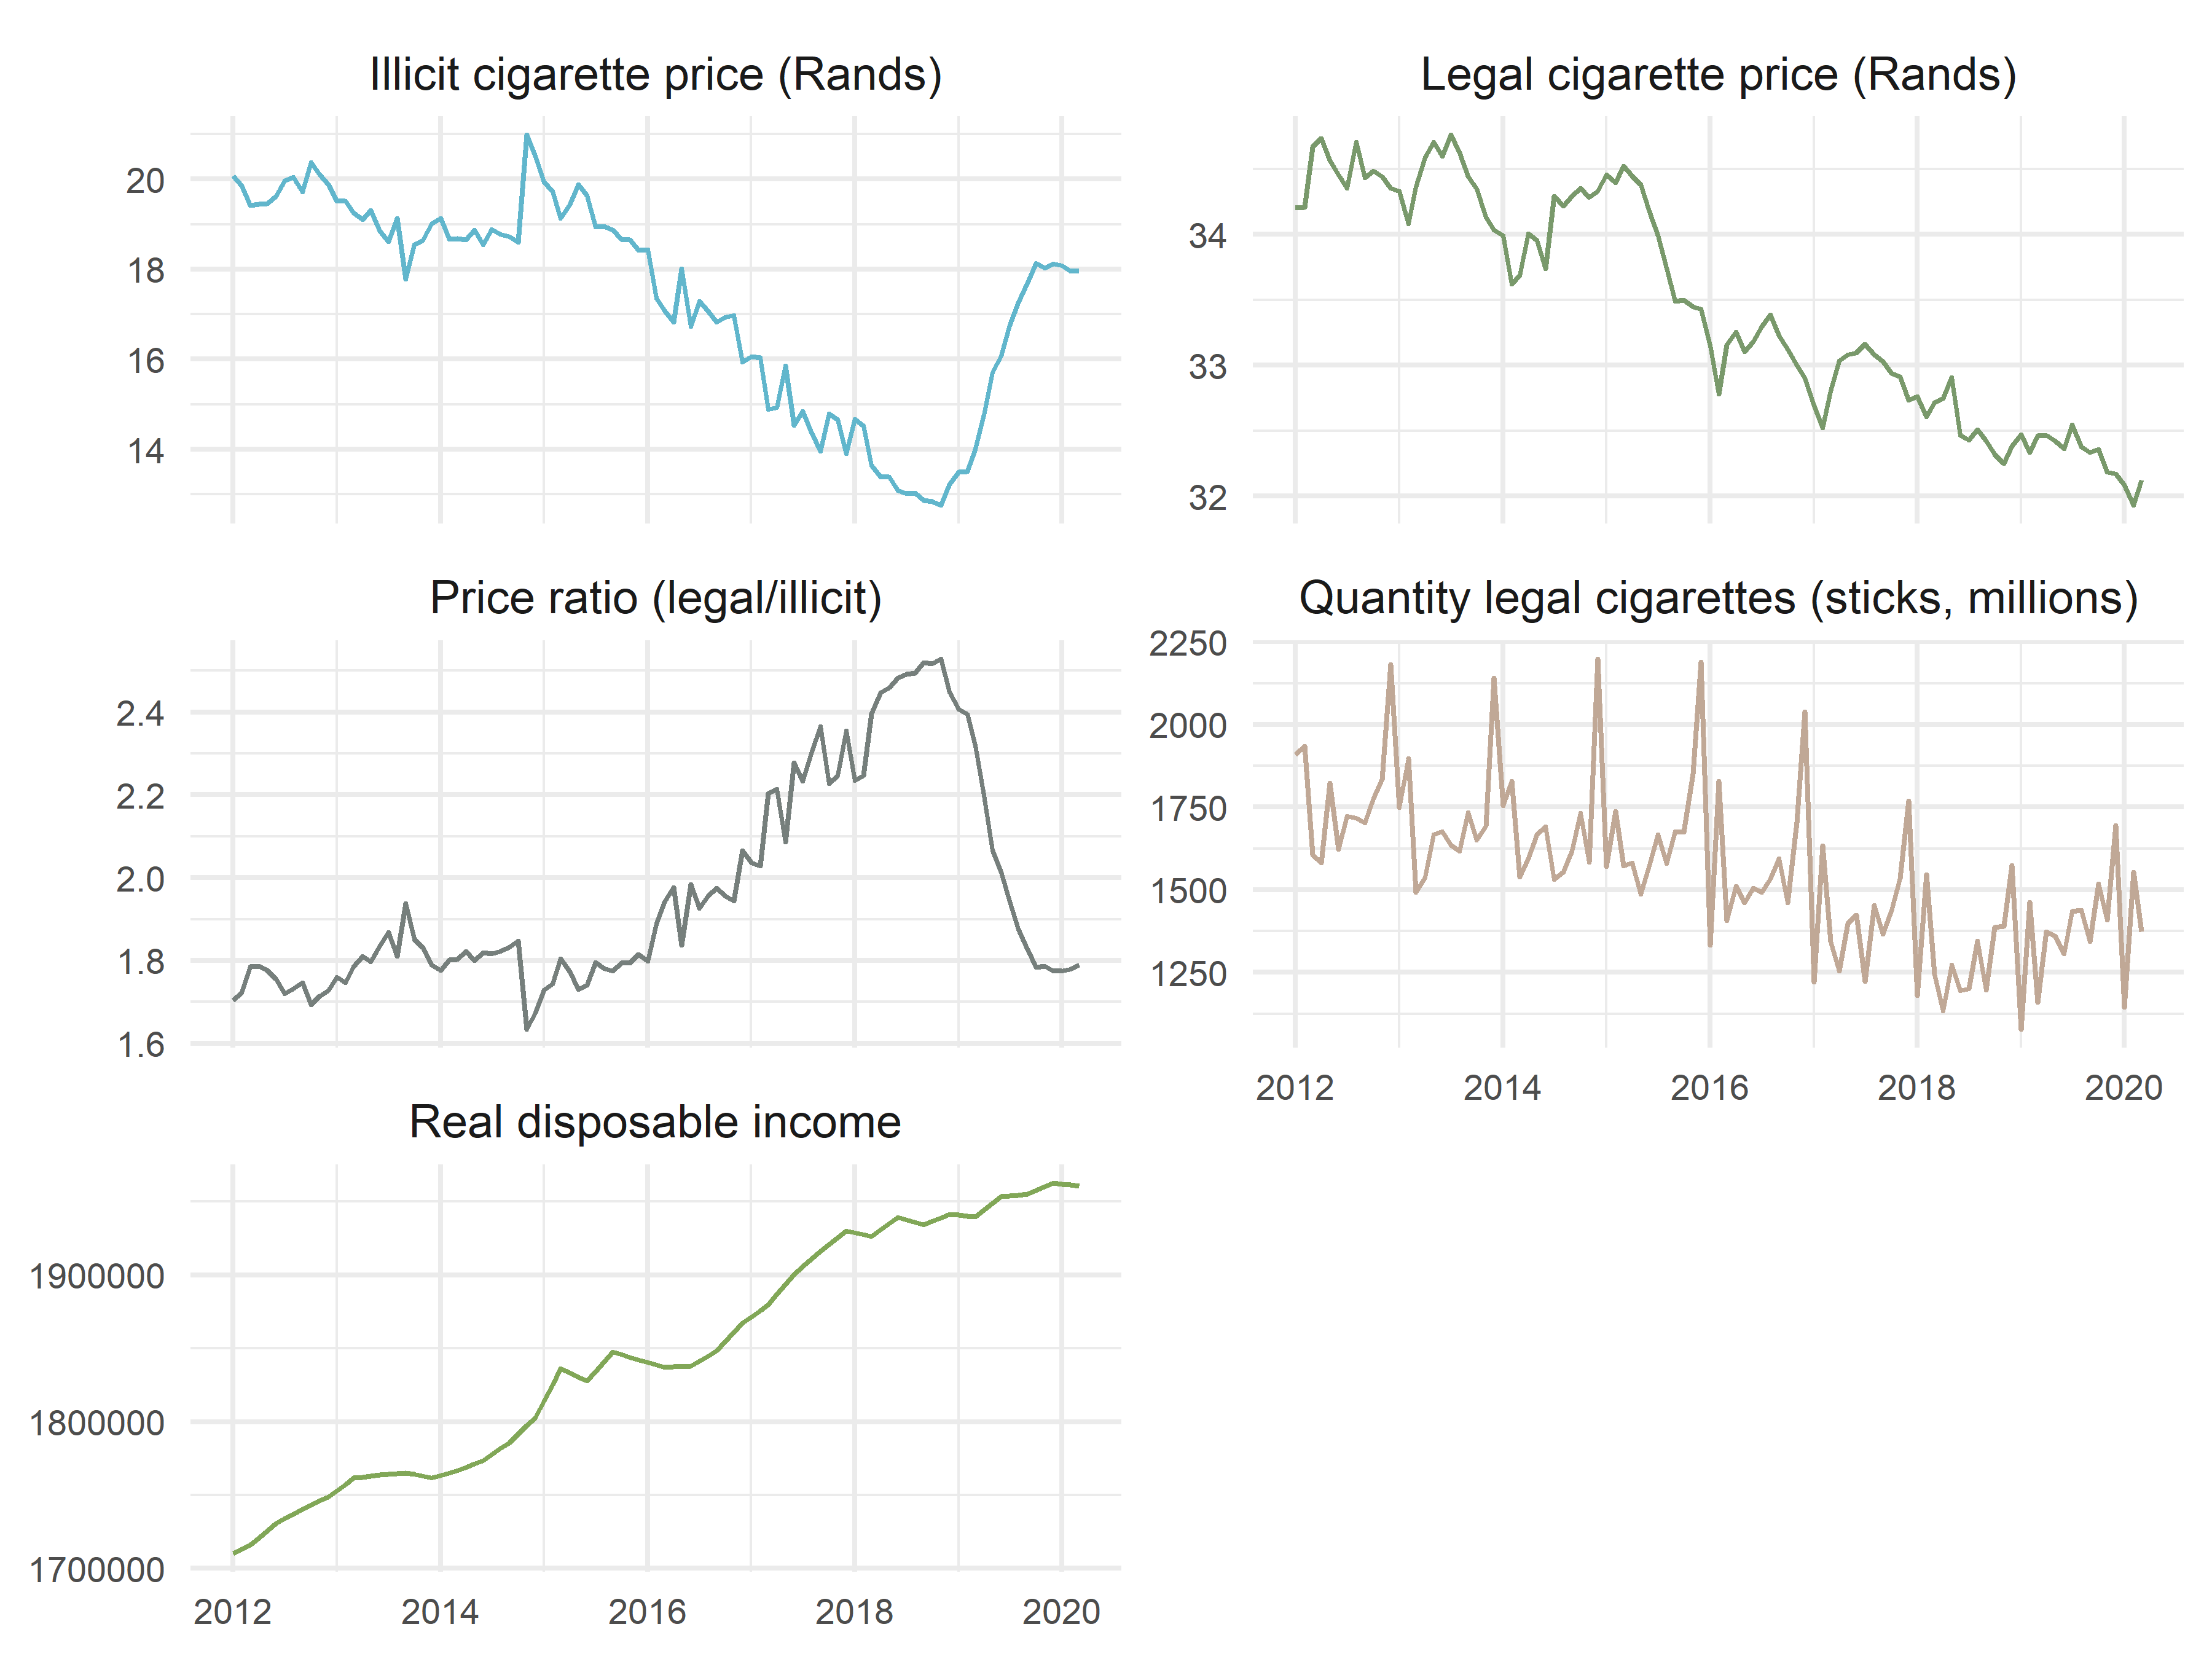
\includegraphics{index_files/figure-latex/graphs-1} 

}

\caption{Plot for variables at levels \label{fig:plot}}\label{fig:graphs}
\end{figure}

\hypertarget{stationarity-and-cointegration}{%
\section{\texorpdfstring{Stationarity and Cointegration
\label{Cointegrate}}{Stationarity and Cointegration }}\label{stationarity-and-cointegration}}

To test whether the series are stationary, three tests were employed:
the Augmented Dickey-Fuller (ADF), and Phillip-Perron (PP) unit root
tests, and the Kwiatkowski--Phillips--Schmidt--Shin (KPSS) stationarity
test. The results of the ADF and PP tests in figures \ref{tab:adf} and
\ref{tab:pp} (presented in appendix \ref{appendixA}) show that the log
of the real price ratio and the log of real per capita disposable income
series are non-stationary at the 5\% level of significance.

Both the ADF and PP tests reject the null hypothesis that the log of
quantity of legal cigarettes consumed contains a unit root at a 5\%
level of significance. The ADF test p-values at a 5\% significance level
for the quantity of legal cigarettes, price ratio, and disposable income
are 0.01, -1.44, and 0.81 respectively. The PP test p-values are 0.01,
-2.54, and 0.412 respectively. The KPSS test (figure \ref{tab:kp})
rejected the null hypothesis of stationarity for all three variables
with a p-value of 0.01 for each variable. Based on the KPSS test, each
one of the variables is assumed to be non-stationary in levels.

However, after first differencing each of the series, all three tests
indicate that the variables are stationary at a 5\% level of
significance. The ADF and PP tests reject the null hypothesis that the
series contain a unit root after they have been differenced, as shown in
tables \ref{adfdiff} and \ref{ppdiff}. The KPSS test fails to reject the
null hypothesis of stationarity for the differenced series with p-values
of 0.1 for every variabe as shown in table \ref{kpssdiff}. Given that
the series are non-stationary in levels and are stationary in first
differences, a cointegration approach can be used to check whether a
long-run relationship exists among the variables.

To test for conintegrating relationships, two tests were employed: the
Johansen Trace test for Cointegration, and the Johansen Maximum
Eigenvalue test for Cointegration.

The Johansen Trace Test for Cointegration indicates that there is one
cointegrating vector. As shown in table \ref{trace}, the test statistic
of 44.1 is larger than 41.1 (the critical value at a 1\% level of
significance). Thus, the null hypothesis is rejected, where the null
hypothesis is that there are zero cointegrating vectors. However, the
test statistic 10.2 is lower than 17.9 (the critical value at a 10\%
level of significance). This means that the null hypothesis cannot be
rejected even at a 10\% signicance level, where the null hypothesis is
that there is 1 or fewer cointegrating vectors.

The results of the Johansen Maximum Eigenvalue test are presented in
table \ref{eigen}. Similar to the Trace test, the Maximum Eigenvalue
test shows that there is a single cointegrating vector. The test
statistic 33.9 exceeds the critical value of 26.8 at a 1\% level of
significance. Therefore the null hypothesis - that there is no
conintegration - is rejected at a 1\% significance level. However, the
null hypothesis that there is 1 or fewer cointegrating relationships
cannot be rejected, even at a 10\% significance level. Here, the test
statistics of 8.48 lies below the 10\% critical value of 13.8.

\hypertarget{vector-error-correction-model}{%
\section{\texorpdfstring{Vector Error Correction Model
\label{vecm}}{Vector Error Correction Model }}\label{vector-error-correction-model}}

The price ratio captures a relative change of the legal price compared
to the illicit price. If the ratio shrinks, it indicates that the cost
of legal cigarettes decreased relative to the cost of illicit
cigarettes. There should be a negative long run relationship between the
price ratio and the quantity of legal cigarettes. There should be a
positive sign for the cointegrating relationship, which there is. The
coefficient for the real disposable income variable should be negative
for the long-run relationship (so that the reverse sign is positive);
whereas the sign is positive in the Vecm results below.

 
  \providecommand{\huxb}[2]{\arrayrulecolor[RGB]{#1}\global\arrayrulewidth=#2pt}
  \providecommand{\huxvb}[2]{\color[RGB]{#1}\vrule width #2pt}
  \providecommand{\huxtpad}[1]{\rule{0pt}{#1}}
  \providecommand{\huxbpad}[1]{\rule[-#1]{0pt}{#1}}

\begin{table}[ht]
\begin{centerbox}
\begin{threeparttable}
\captionsetup{justification=centering,singlelinecheck=off}
\caption{Long run coefficient}
 \label{tab:VecmResults}
\setlength{\tabcolsep}{0pt}
\begin{tabular}{l}


\hhline{>{\huxb{0, 0, 0}{0.4}}-}
\arrayrulecolor{black}

\multicolumn{1}{!{\huxvb{0, 0, 0}{0}}r!{\huxvb{0, 0, 0}{0}}}{\huxtpad{2pt + 1em}\raggedleft \hspace{2pt} \textbf{{\fontsize{10pt}{12pt}\selectfont r1}} \hspace{2pt}\huxbpad{2pt}} \tabularnewline[-0.5pt]


\hhline{>{\huxb{0, 0, 0}{0.4}}-}
\arrayrulecolor{black}

\multicolumn{1}{!{\huxvb{0, 0, 0}{0}}r!{\huxvb{0, 0, 0}{0}}}{\huxtpad{2pt + 1em}\raggedleft \hspace{2pt} {\fontsize{10pt}{12pt}\selectfont 1\hphantom{0}\hphantom{0}\hphantom{0}\hphantom{0}} \hspace{2pt}\huxbpad{2pt}} \tabularnewline[-0.5pt]


\hhline{}
\arrayrulecolor{black}

\multicolumn{1}{!{\huxvb{0, 0, 0}{0}}r!{\huxvb{0, 0, 0}{0}}}{\huxtpad{2pt + 1em}\raggedleft \hspace{2pt} {\fontsize{10pt}{12pt}\selectfont 0.398} \hspace{2pt}\huxbpad{2pt}} \tabularnewline[-0.5pt]


\hhline{}
\arrayrulecolor{black}

\multicolumn{1}{!{\huxvb{0, 0, 0}{0}}r!{\huxvb{0, 0, 0}{0}}}{\huxtpad{2pt + 1em}\raggedleft \hspace{2pt} {\fontsize{10pt}{12pt}\selectfont 1.5\hphantom{0}\hphantom{0}} \hspace{2pt}\huxbpad{2pt}} \tabularnewline[-0.5pt]


\hhline{>{\huxb{0, 0, 0}{0.4}}-}
\arrayrulecolor{black}
\end{tabular}
\end{threeparttable}\par\end{centerbox}

\end{table}
 

 
  \providecommand{\huxb}[2]{\arrayrulecolor[RGB]{#1}\global\arrayrulewidth=#2pt}
  \providecommand{\huxvb}[2]{\color[RGB]{#1}\vrule width #2pt}
  \providecommand{\huxtpad}[1]{\rule{0pt}{#1}}
  \providecommand{\huxbpad}[1]{\rule[-#1]{0pt}{#1}}

\begin{table}[ht]
\begin{centerbox}
\begin{threeparttable}
\captionsetup{justification=centering,singlelinecheck=off}
\caption{Short tunrun coefficient}
 \label{tab:VecmResults}
\setlength{\tabcolsep}{0pt}
\begin{tabular}{l l l l l}


\hhline{>{\huxb{0, 0, 0}{0.4}}->{\huxb{0, 0, 0}{0.4}}->{\huxb{0, 0, 0}{0.4}}->{\huxb{0, 0, 0}{0.4}}->{\huxb{0, 0, 0}{0.4}}-}
\arrayrulecolor{black}

\multicolumn{1}{!{\huxvb{0, 0, 0}{0}}l!{\huxvb{0, 0, 0}{0}}}{\huxtpad{2pt + 1em}\raggedright \hspace{2pt} \textbf{{\fontsize{10pt}{12pt}\selectfont ECT}} \hspace{2pt}\huxbpad{2pt}} &
\multicolumn{1}{l!{\huxvb{0, 0, 0}{0}}}{\huxtpad{2pt + 1em}\raggedright \hspace{2pt} \textbf{{\fontsize{10pt}{12pt}\selectfont Intercept}} \hspace{2pt}\huxbpad{2pt}} &
\multicolumn{1}{l!{\huxvb{0, 0, 0}{0}}}{\huxtpad{2pt + 1em}\raggedright \hspace{2pt} \textbf{{\fontsize{10pt}{12pt}\selectfont QDP -1}} \hspace{2pt}\huxbpad{2pt}} &
\multicolumn{1}{l!{\huxvb{0, 0, 0}{0}}}{\huxtpad{2pt + 1em}\raggedright \hspace{2pt} \textbf{{\fontsize{10pt}{12pt}\selectfont PRATIO -1}} \hspace{2pt}\huxbpad{2pt}} &
\multicolumn{1}{l!{\huxvb{0, 0, 0}{0}}}{\huxtpad{2pt + 1em}\raggedright \hspace{2pt} \textbf{{\fontsize{10pt}{12pt}\selectfont REAL -1}} \hspace{2pt}\huxbpad{2pt}} \tabularnewline[-0.5pt]


\hhline{>{\huxb{0, 0, 0}{0.4}}->{\huxb{0, 0, 0}{0.4}}->{\huxb{0, 0, 0}{0.4}}->{\huxb{0, 0, 0}{0.4}}->{\huxb{0, 0, 0}{0.4}}-}
\arrayrulecolor{black}

\multicolumn{1}{!{\huxvb{0, 0, 0}{0}}l!{\huxvb{0, 0, 0}{0}}}{\huxtpad{2pt + 1em}\raggedright \hspace{2pt} {\fontsize{10pt}{12pt}\selectfont -0.9443(0.1526)***} \hspace{2pt}\huxbpad{2pt}} &
\multicolumn{1}{l!{\huxvb{0, 0, 0}{0}}}{\huxtpad{2pt + 1em}\raggedright \hspace{2pt} {\fontsize{10pt}{12pt}\selectfont 27.7687(4.4890)***} \hspace{2pt}\huxbpad{2pt}} &
\multicolumn{1}{l!{\huxvb{0, 0, 0}{0}}}{\huxtpad{2pt + 1em}\raggedright \hspace{2pt} {\fontsize{10pt}{12pt}\selectfont -0.1910(0.0964).  } \hspace{2pt}\huxbpad{2pt}} &
\multicolumn{1}{l!{\huxvb{0, 0, 0}{0}}}{\huxtpad{2pt + 1em}\raggedright \hspace{2pt} {\fontsize{10pt}{12pt}\selectfont -0.9964(0.3181)** } \hspace{2pt}\huxbpad{2pt}} &
\multicolumn{1}{l!{\huxvb{0, 0, 0}{0}}}{\huxtpad{2pt + 1em}\raggedright \hspace{2pt} {\fontsize{10pt}{12pt}\selectfont 2.3116(4.4102)    } \hspace{2pt}\huxbpad{2pt}} \tabularnewline[-0.5pt]


\hhline{}
\arrayrulecolor{black}

\multicolumn{1}{!{\huxvb{0, 0, 0}{0}}l!{\huxvb{0, 0, 0}{0}}}{\huxtpad{2pt + 1em}\raggedright \hspace{2pt} {\fontsize{10pt}{12pt}\selectfont -0.0077(0.0511)    } \hspace{2pt}\huxbpad{2pt}} &
\multicolumn{1}{l!{\huxvb{0, 0, 0}{0}}}{\huxtpad{2pt + 1em}\raggedright \hspace{2pt} {\fontsize{10pt}{12pt}\selectfont 0.2274(1.5033)    } \hspace{2pt}\huxbpad{2pt}} &
\multicolumn{1}{l!{\huxvb{0, 0, 0}{0}}}{\huxtpad{2pt + 1em}\raggedright \hspace{2pt} {\fontsize{10pt}{12pt}\selectfont 0.0148(0.0323)    } \hspace{2pt}\huxbpad{2pt}} &
\multicolumn{1}{l!{\huxvb{0, 0, 0}{0}}}{\huxtpad{2pt + 1em}\raggedright \hspace{2pt} {\fontsize{10pt}{12pt}\selectfont -0.1555(0.1065)    } \hspace{2pt}\huxbpad{2pt}} &
\multicolumn{1}{l!{\huxvb{0, 0, 0}{0}}}{\huxtpad{2pt + 1em}\raggedright \hspace{2pt} {\fontsize{10pt}{12pt}\selectfont 0.3575(1.4769)    } \hspace{2pt}\huxbpad{2pt}} \tabularnewline[-0.5pt]


\hhline{}
\arrayrulecolor{black}

\multicolumn{1}{!{\huxvb{0, 0, 0}{0}}l!{\huxvb{0, 0, 0}{0}}}{\huxtpad{2pt + 1em}\raggedright \hspace{2pt} {\fontsize{10pt}{12pt}\selectfont 0.0010(0.0030)    } \hspace{2pt}\huxbpad{2pt}} &
\multicolumn{1}{l!{\huxvb{0, 0, 0}{0}}}{\huxtpad{2pt + 1em}\raggedright \hspace{2pt} {\fontsize{10pt}{12pt}\selectfont -0.0299(0.0870)    } \hspace{2pt}\huxbpad{2pt}} &
\multicolumn{1}{l!{\huxvb{0, 0, 0}{0}}}{\huxtpad{2pt + 1em}\raggedright \hspace{2pt} {\fontsize{10pt}{12pt}\selectfont 0.0004(0.0019)    } \hspace{2pt}\huxbpad{2pt}} &
\multicolumn{1}{l!{\huxvb{0, 0, 0}{0}}}{\huxtpad{2pt + 1em}\raggedright \hspace{2pt} {\fontsize{10pt}{12pt}\selectfont 0.0019(0.0062)    } \hspace{2pt}\huxbpad{2pt}} &
\multicolumn{1}{l!{\huxvb{0, 0, 0}{0}}}{\huxtpad{2pt + 1em}\raggedright \hspace{2pt} {\fontsize{10pt}{12pt}\selectfont 0.5833(0.0855)***} \hspace{2pt}\huxbpad{2pt}} \tabularnewline[-0.5pt]


\hhline{>{\huxb{0, 0, 0}{0.4}}->{\huxb{0, 0, 0}{0.4}}->{\huxb{0, 0, 0}{0.4}}->{\huxb{0, 0, 0}{0.4}}->{\huxb{0, 0, 0}{0.4}}-}
\arrayrulecolor{black}
\end{tabular}
\end{threeparttable}\par\end{centerbox}

\end{table}
 

If the real disposable income variable is excluded then the Vecm results
are as follows. The coefficient for

 
  \providecommand{\huxb}[2]{\arrayrulecolor[RGB]{#1}\global\arrayrulewidth=#2pt}
  \providecommand{\huxvb}[2]{\color[RGB]{#1}\vrule width #2pt}
  \providecommand{\huxtpad}[1]{\rule{0pt}{#1}}
  \providecommand{\huxbpad}[1]{\rule[-#1]{0pt}{#1}}

\begin{table}[ht]
\begin{centerbox}
\begin{threeparttable}
 \label{tab:VecmResultsSingle}
\setlength{\tabcolsep}{0pt}
\begin{tabularx}{0.9\textwidth}{p{0.45\textwidth} p{0.45\textwidth}}


\hhline{}
\arrayrulecolor{black}

\multicolumn{1}{!{\huxvb{0, 0, 0}{0}}p{0.45\textwidth}!{\huxvb{0, 0, 0}{0}}}{\hspace{2pt}\parbox[b]{0.45\textwidth-2pt-2pt}{\huxtpad{6pt + 1em}\raggedright \textbf{1.00}\huxbpad{6pt}}} &
\multicolumn{1}{p{0.45\textwidth}!{\huxvb{0, 0, 0}{0}}}{\hspace{2pt}\parbox[b]{0.45\textwidth-2pt-2pt}{\huxtpad{6pt + 1em}\raggedleft \textbf{r1.00}\huxbpad{6pt}}} \tabularnewline[-0.5pt]


\hhline{>{\huxb{0, 0, 0}{0.4}}->{\huxb{0, 0, 0}{0.4}}-}
\arrayrulecolor{black}

\multicolumn{1}{!{\huxvb{0, 0, 0}{0}}p{0.45\textwidth}!{\huxvb{0, 0, 0}{0}}}{\hspace{2pt}\parbox[b]{0.45\textwidth-2pt-2pt}{\huxtpad{6pt + 1em}\raggedright QDP\huxbpad{6pt}}} &
\multicolumn{1}{p{0.45\textwidth}!{\huxvb{0, 0, 0}{0}}}{\hspace{2pt}\parbox[b]{0.45\textwidth-2pt-2pt}{\huxtpad{6pt + 1em}\raggedleft 1.00\huxbpad{6pt}}} \tabularnewline[-0.5pt]


\hhline{}
\arrayrulecolor{black}

\multicolumn{1}{!{\huxvb{0, 0, 0}{0}}p{0.45\textwidth}!{\huxvb{0, 0, 0}{0}}}{\hspace{2pt}\parbox[b]{0.45\textwidth-2pt-2pt}{\huxtpad{6pt + 1em}\raggedright PRATIO\huxbpad{6pt}}} &
\multicolumn{1}{p{0.45\textwidth}!{\huxvb{0, 0, 0}{0}}}{\hspace{2pt}\parbox[b]{0.45\textwidth-2pt-2pt}{\huxtpad{6pt + 1em}\raggedleft 0.75\huxbpad{6pt}}} \tabularnewline[-0.5pt]


\hhline{}
\arrayrulecolor{black}
\end{tabularx}
\end{threeparttable}\par\end{centerbox}

\end{table}
 

 
  \providecommand{\huxb}[2]{\arrayrulecolor[RGB]{#1}\global\arrayrulewidth=#2pt}
  \providecommand{\huxvb}[2]{\color[RGB]{#1}\vrule width #2pt}
  \providecommand{\huxtpad}[1]{\rule{0pt}{#1}}
  \providecommand{\huxbpad}[1]{\rule[-#1]{0pt}{#1}}

\begin{table}[ht]
\begin{centerbox}
\begin{threeparttable}
 \label{tab:VecmResultsSingle}
\setlength{\tabcolsep}{0pt}
\begin{tabularx}{0.9\textwidth}{p{0.18\textwidth} p{0.18\textwidth} p{0.18\textwidth} p{0.18\textwidth} p{0.18\textwidth}}


\hhline{}
\arrayrulecolor{black}

\multicolumn{1}{!{\huxvb{0, 0, 0}{0}}p{0.18\textwidth}!{\huxvb{0, 0, 0}{0}}}{\hspace{2pt}\parbox[b]{0.18\textwidth-2pt-2pt}{\huxtpad{6pt + 1em}\raggedright \textbf{1.00}\huxbpad{6pt}}} &
\multicolumn{1}{p{0.18\textwidth}!{\huxvb{0, 0, 0}{0}}}{\hspace{2pt}\parbox[b]{0.18\textwidth-2pt-2pt}{\huxtpad{6pt + 1em}\raggedleft \textbf{ECT}\huxbpad{6pt}}} &
\multicolumn{1}{p{0.18\textwidth}!{\huxvb{0, 0, 0}{0}}}{\hspace{2pt}\parbox[b]{0.18\textwidth-2pt-2pt}{\huxtpad{6pt + 1em}\raggedright \textbf{Intercept}\huxbpad{6pt}}} &
\multicolumn{1}{p{0.18\textwidth}!{\huxvb{0, 0, 0}{0}}}{\hspace{2pt}\parbox[b]{0.18\textwidth-2pt-2pt}{\huxtpad{6pt + 1em}\raggedright \textbf{QDP -1.00}\huxbpad{6pt}}} &
\multicolumn{1}{p{0.18\textwidth}!{\huxvb{0, 0, 0}{0}}}{\hspace{2pt}\parbox[b]{0.18\textwidth-2pt-2pt}{\huxtpad{6pt + 1em}\raggedright \textbf{PRATIO -1.00}\huxbpad{6pt}}} \tabularnewline[-0.5pt]


\hhline{>{\huxb{0, 0, 0}{0.4}}->{\huxb{0, 0, 0}{0.4}}->{\huxb{0, 0, 0}{0.4}}->{\huxb{0, 0, 0}{0.4}}->{\huxb{0, 0, 0}{0.4}}-}
\arrayrulecolor{black}

\multicolumn{1}{!{\huxvb{0, 0, 0}{0}}p{0.18\textwidth}!{\huxvb{0, 0, 0}{0}}}{\hspace{2pt}\parbox[b]{0.18\textwidth-2pt-2pt}{\huxtpad{6pt + 1em}\raggedright Equation QDP\huxbpad{6pt}}} &
\multicolumn{1}{p{0.18\textwidth}!{\huxvb{0, 0, 0}{0}}}{\hspace{2pt}\parbox[b]{0.18\textwidth-2pt-2pt}{\huxtpad{6pt + 1em}\raggedleft -0.64(0.14)***\huxbpad{6pt}}} &
\multicolumn{1}{p{0.18\textwidth}!{\huxvb{0, 0, 0}{0}}}{\hspace{2pt}\parbox[b]{0.18\textwidth-2pt-2pt}{\huxtpad{6pt + 1em}\raggedright 5.05(1.08)***\huxbpad{6pt}}} &
\multicolumn{1}{p{0.18\textwidth}!{\huxvb{0, 0, 0}{0}}}{\hspace{2pt}\parbox[b]{0.18\textwidth-2pt-2pt}{\huxtpad{6pt + 1em}\raggedright -0.35(0.09)***\huxbpad{6pt}}} &
\multicolumn{1}{p{0.18\textwidth}!{\huxvb{0, 0, 0}{0}}}{\hspace{2pt}\parbox[b]{0.18\textwidth-2pt-2pt}{\huxtpad{6pt + 1em}\raggedright -0.91(0.35)*  \huxbpad{6pt}}} \tabularnewline[-0.5pt]


\hhline{}
\arrayrulecolor{black}

\multicolumn{1}{!{\huxvb{0, 0, 0}{0}}p{0.18\textwidth}!{\huxvb{0, 0, 0}{0}}}{\hspace{2pt}\parbox[b]{0.18\textwidth-2pt-2pt}{\huxtpad{6pt + 1em}\raggedright Equation PRATIO\huxbpad{6pt}}} &
\multicolumn{1}{p{0.18\textwidth}!{\huxvb{0, 0, 0}{0}}}{\hspace{2pt}\parbox[b]{0.18\textwidth-2pt-2pt}{\huxtpad{6pt + 1em}\raggedleft 0.01(0.04)    \huxbpad{6pt}}} &
\multicolumn{1}{p{0.18\textwidth}!{\huxvb{0, 0, 0}{0}}}{\hspace{2pt}\parbox[b]{0.18\textwidth-2pt-2pt}{\huxtpad{6pt + 1em}\raggedright -0.07(0.34)    \huxbpad{6pt}}} &
\multicolumn{1}{p{0.18\textwidth}!{\huxvb{0, 0, 0}{0}}}{\hspace{2pt}\parbox[b]{0.18\textwidth-2pt-2pt}{\huxtpad{6pt + 1em}\raggedright 0.01(0.03)    \huxbpad{6pt}}} &
\multicolumn{1}{p{0.18\textwidth}!{\huxvb{0, 0, 0}{0}}}{\hspace{2pt}\parbox[b]{0.18\textwidth-2pt-2pt}{\huxtpad{6pt + 1em}\raggedright -0.17(0.11)    \huxbpad{6pt}}} \tabularnewline[-0.5pt]


\hhline{}
\arrayrulecolor{black}
\end{tabularx}
\end{threeparttable}\par\end{centerbox}

\end{table}
 

\hypertarget{residual-testing}{%
\section{\texorpdfstring{Residual Testing
\label{residuals}}{Residual Testing }}\label{residual-testing}}

\hypertarget{analysis}{%
\chapter{\texorpdfstring{Analysis
\label{analysis}}{Analysis }}\label{analysis}}

\hypertarget{conclusion}{%
\chapter{\texorpdfstring{Conclusion
\label{conclusion}}{Conclusion }}\label{conclusion}}

\appendix
\appendixpage

\hypertarget{stationarity-testing}{%
\chapter{\texorpdfstring{Stationarity Testing
\label{appendixA}}{Stationarity Testing }}\label{stationarity-testing}}

 
  \providecommand{\huxb}[2]{\arrayrulecolor[RGB]{#1}\global\arrayrulewidth=#2pt}
  \providecommand{\huxvb}[2]{\color[RGB]{#1}\vrule width #2pt}
  \providecommand{\huxtpad}[1]{\rule{0pt}{#1}}
  \providecommand{\huxbpad}[1]{\rule[-#1]{0pt}{#1}}

\begin{table}[ht]
\begin{centerbox}
\begin{threeparttable}
\captionsetup{justification=centering,singlelinecheck=off}
\caption{Augmented Dickey Fuller Tests \label{tab:adf}}
 \label{tab:ADFResults}
\setlength{\tabcolsep}{0pt}
\begin{tabular}{l l l l}


\hhline{>{\huxb{255, 255, 255}{0.4}}->{\huxb{0, 0, 0}{0.4}}->{\huxb{0, 0, 0}{0.4}}->{\huxb{0, 0, 0}{0.4}}-}
\arrayrulecolor{black}

\multicolumn{1}{!{\huxvb{0, 0, 0}{0}}l!{\huxvb{0, 0, 0}{0}}}{\huxtpad{3pt + 1em}\raggedright \hspace{3pt} {\fontsize{10pt}{12pt}\selectfont } \hspace{2pt}\huxbpad{2pt}} &
\multicolumn{1}{l!{\huxvb{0, 0, 0}{0}}}{\huxtpad{3pt + 1em}\raggedright \hspace{2pt} \textbf{{\fontsize{10pt}{12pt}\selectfont Statistic}} \hspace{2pt}\huxbpad{2pt}} &
\multicolumn{1}{l!{\huxvb{0, 0, 0}{0}}}{\huxtpad{3pt + 1em}\raggedright \hspace{2pt} \textbf{{\fontsize{10pt}{12pt}\selectfont p-value}} \hspace{2pt}\huxbpad{2pt}} &
\multicolumn{1}{l!{\huxvb{0, 0, 0}{0}}}{\huxtpad{3pt + 1em}\raggedright \hspace{2pt} \textbf{{\fontsize{10pt}{12pt}\selectfont Alternative}} \hspace{3pt}\huxbpad{2pt}} \tabularnewline[-0.5pt]


\hhline{>{\huxb{255, 255, 255}{0.4}}->{\huxb{0, 0, 0}{0.4}}->{\huxb{0, 0, 0}{0.4}}->{\huxb{0, 0, 0}{0.4}}-}
\arrayrulecolor{black}

\multicolumn{1}{!{\huxvb{0, 0, 0}{0}}l!{\huxvb{0, 0, 0}{0}}}{\huxtpad{2pt + 1em}\raggedright \hspace{3pt} {\fontsize{10pt}{12pt}\selectfont Quantity legal cigarettes} \hspace{2pt}\huxbpad{2pt}} &
\multicolumn{1}{l!{\huxvb{0, 0, 0}{0}}}{\huxtpad{2pt + 1em}\raggedright \hspace{2pt} {\fontsize{10pt}{12pt}\selectfont -4.67} \hspace{2pt}\huxbpad{2pt}} &
\multicolumn{1}{l!{\huxvb{0, 0, 0}{0}}}{\huxtpad{2pt + 1em}\raggedright \hspace{2pt} {\fontsize{10pt}{12pt}\selectfont 0.01} \hspace{2pt}\huxbpad{2pt}} &
\multicolumn{1}{l!{\huxvb{0, 0, 0}{0}}}{\huxtpad{2pt + 1em}\raggedright \hspace{2pt} {\fontsize{10pt}{12pt}\selectfont stationary} \hspace{3pt}\huxbpad{2pt}} \tabularnewline[-0.5pt]


\hhline{}
\arrayrulecolor{black}

\multicolumn{1}{!{\huxvb{0, 0, 0}{0}}l!{\huxvb{0, 0, 0}{0}}}{\huxtpad{2pt + 1em}\raggedright \hspace{3pt} {\fontsize{10pt}{12pt}\selectfont Price ratio} \hspace{2pt}\huxbpad{2pt}} &
\multicolumn{1}{l!{\huxvb{0, 0, 0}{0}}}{\huxtpad{2pt + 1em}\raggedright \hspace{2pt} {\fontsize{10pt}{12pt}\selectfont -1.44} \hspace{2pt}\huxbpad{2pt}} &
\multicolumn{1}{l!{\huxvb{0, 0, 0}{0}}}{\huxtpad{2pt + 1em}\raggedright \hspace{2pt} {\fontsize{10pt}{12pt}\selectfont 0.808} \hspace{2pt}\huxbpad{2pt}} &
\multicolumn{1}{l!{\huxvb{0, 0, 0}{0}}}{\huxtpad{2pt + 1em}\raggedright \hspace{2pt} {\fontsize{10pt}{12pt}\selectfont stationary} \hspace{3pt}\huxbpad{2pt}} \tabularnewline[-0.5pt]


\hhline{}
\arrayrulecolor{black}

\multicolumn{1}{!{\huxvb{0, 0, 0}{0}}l!{\huxvb{0, 0, 0}{0}}}{\huxtpad{2pt + 1em}\raggedright \hspace{3pt} {\fontsize{10pt}{12pt}\selectfont Disposable income} \hspace{2pt}\huxbpad{3pt}} &
\multicolumn{1}{l!{\huxvb{0, 0, 0}{0}}}{\huxtpad{2pt + 1em}\raggedright \hspace{2pt} {\fontsize{10pt}{12pt}\selectfont -3.31} \hspace{2pt}\huxbpad{3pt}} &
\multicolumn{1}{l!{\huxvb{0, 0, 0}{0}}}{\huxtpad{2pt + 1em}\raggedright \hspace{2pt} {\fontsize{10pt}{12pt}\selectfont 0.0739} \hspace{2pt}\huxbpad{3pt}} &
\multicolumn{1}{l!{\huxvb{0, 0, 0}{0}}}{\huxtpad{2pt + 1em}\raggedright \hspace{2pt} {\fontsize{10pt}{12pt}\selectfont stationary} \hspace{3pt}\huxbpad{3pt}} \tabularnewline[-0.5pt]


\hhline{>{\huxb{0, 0, 0}{0.4}}->{\huxb{0, 0, 0}{0.4}}->{\huxb{0, 0, 0}{0.4}}->{\huxb{0, 0, 0}{0.4}}-}
\arrayrulecolor{black}
\end{tabular}
\end{threeparttable}\par\end{centerbox}

\end{table}
 

 
  \providecommand{\huxb}[2]{\arrayrulecolor[RGB]{#1}\global\arrayrulewidth=#2pt}
  \providecommand{\huxvb}[2]{\color[RGB]{#1}\vrule width #2pt}
  \providecommand{\huxtpad}[1]{\rule{0pt}{#1}}
  \providecommand{\huxbpad}[1]{\rule[-#1]{0pt}{#1}}

\begin{table}[ht]
\begin{centerbox}
\begin{threeparttable}
\captionsetup{justification=centering,singlelinecheck=off}
\caption{Phillips-Perron Unit Root Test \label{tab:pp}}
 \label{tab:PPResults}
\setlength{\tabcolsep}{0pt}
\begin{tabular}{l l l l}


\hhline{>{\huxb{255, 255, 255}{0.4}}->{\huxb{0, 0, 0}{0.4}}->{\huxb{0, 0, 0}{0.4}}->{\huxb{0, 0, 0}{0.4}}-}
\arrayrulecolor{black}

\multicolumn{1}{!{\huxvb{0, 0, 0}{0}}l!{\huxvb{0, 0, 0}{0}}}{\huxtpad{3pt + 1em}\raggedright \hspace{3pt} {\fontsize{10pt}{12pt}\selectfont } \hspace{2pt}\huxbpad{2pt}} &
\multicolumn{1}{l!{\huxvb{0, 0, 0}{0}}}{\huxtpad{3pt + 1em}\raggedright \hspace{2pt} \textbf{{\fontsize{10pt}{12pt}\selectfont Statistic}} \hspace{2pt}\huxbpad{2pt}} &
\multicolumn{1}{l!{\huxvb{0, 0, 0}{0}}}{\huxtpad{3pt + 1em}\raggedright \hspace{2pt} \textbf{{\fontsize{10pt}{12pt}\selectfont p-value}} \hspace{2pt}\huxbpad{2pt}} &
\multicolumn{1}{l!{\huxvb{0, 0, 0}{0}}}{\huxtpad{3pt + 1em}\raggedright \hspace{2pt} \textbf{{\fontsize{10pt}{12pt}\selectfont Alternative}} \hspace{3pt}\huxbpad{2pt}} \tabularnewline[-0.5pt]


\hhline{>{\huxb{255, 255, 255}{0.4}}->{\huxb{0, 0, 0}{0.4}}->{\huxb{0, 0, 0}{0.4}}->{\huxb{0, 0, 0}{0.4}}-}
\arrayrulecolor{black}

\multicolumn{1}{!{\huxvb{0, 0, 0}{0}}l!{\huxvb{0, 0, 0}{0}}}{\huxtpad{2pt + 1em}\raggedright \hspace{3pt} {\fontsize{10pt}{12pt}\selectfont Quantity legal cigarettes} \hspace{2pt}\huxbpad{2pt}} &
\multicolumn{1}{l!{\huxvb{0, 0, 0}{0}}}{\huxtpad{2pt + 1em}\raggedright \hspace{2pt} {\fontsize{10pt}{12pt}\selectfont -119} \hspace{2pt}\huxbpad{2pt}} &
\multicolumn{1}{l!{\huxvb{0, 0, 0}{0}}}{\huxtpad{2pt + 1em}\raggedright \hspace{2pt} {\fontsize{10pt}{12pt}\selectfont 0.01} \hspace{2pt}\huxbpad{2pt}} &
\multicolumn{1}{l!{\huxvb{0, 0, 0}{0}}}{\huxtpad{2pt + 1em}\raggedright \hspace{2pt} {\fontsize{10pt}{12pt}\selectfont stationary} \hspace{3pt}\huxbpad{2pt}} \tabularnewline[-0.5pt]


\hhline{}
\arrayrulecolor{black}

\multicolumn{1}{!{\huxvb{0, 0, 0}{0}}l!{\huxvb{0, 0, 0}{0}}}{\huxtpad{2pt + 1em}\raggedright \hspace{3pt} {\fontsize{10pt}{12pt}\selectfont Price ratio} \hspace{2pt}\huxbpad{2pt}} &
\multicolumn{1}{l!{\huxvb{0, 0, 0}{0}}}{\huxtpad{2pt + 1em}\raggedright \hspace{2pt} {\fontsize{10pt}{12pt}\selectfont -2.54} \hspace{2pt}\huxbpad{2pt}} &
\multicolumn{1}{l!{\huxvb{0, 0, 0}{0}}}{\huxtpad{2pt + 1em}\raggedright \hspace{2pt} {\fontsize{10pt}{12pt}\selectfont 0.952} \hspace{2pt}\huxbpad{2pt}} &
\multicolumn{1}{l!{\huxvb{0, 0, 0}{0}}}{\huxtpad{2pt + 1em}\raggedright \hspace{2pt} {\fontsize{10pt}{12pt}\selectfont stationary} \hspace{3pt}\huxbpad{2pt}} \tabularnewline[-0.5pt]


\hhline{}
\arrayrulecolor{black}

\multicolumn{1}{!{\huxvb{0, 0, 0}{0}}l!{\huxvb{0, 0, 0}{0}}}{\huxtpad{2pt + 1em}\raggedright \hspace{3pt} {\fontsize{10pt}{12pt}\selectfont Disposable income} \hspace{2pt}\huxbpad{3pt}} &
\multicolumn{1}{l!{\huxvb{0, 0, 0}{0}}}{\huxtpad{2pt + 1em}\raggedright \hspace{2pt} {\fontsize{10pt}{12pt}\selectfont -12.1} \hspace{2pt}\huxbpad{3pt}} &
\multicolumn{1}{l!{\huxvb{0, 0, 0}{0}}}{\huxtpad{2pt + 1em}\raggedright \hspace{2pt} {\fontsize{10pt}{12pt}\selectfont 0.412} \hspace{2pt}\huxbpad{3pt}} &
\multicolumn{1}{l!{\huxvb{0, 0, 0}{0}}}{\huxtpad{2pt + 1em}\raggedright \hspace{2pt} {\fontsize{10pt}{12pt}\selectfont stationary} \hspace{3pt}\huxbpad{3pt}} \tabularnewline[-0.5pt]


\hhline{>{\huxb{0, 0, 0}{0.4}}->{\huxb{0, 0, 0}{0.4}}->{\huxb{0, 0, 0}{0.4}}->{\huxb{0, 0, 0}{0.4}}-}
\arrayrulecolor{black}
\end{tabular}
\end{threeparttable}\par\end{centerbox}

\end{table}
 

 
  \providecommand{\huxb}[2]{\arrayrulecolor[RGB]{#1}\global\arrayrulewidth=#2pt}
  \providecommand{\huxvb}[2]{\color[RGB]{#1}\vrule width #2pt}
  \providecommand{\huxtpad}[1]{\rule{0pt}{#1}}
  \providecommand{\huxbpad}[1]{\rule[-#1]{0pt}{#1}}

\begin{table}[ht]
\begin{centerbox}
\begin{threeparttable}
\captionsetup{justification=centering,singlelinecheck=off}
\caption{KPSS Unit Root Test \label{tab:kp}}
 \label{tab:KPSSResults}
\setlength{\tabcolsep}{0pt}
\begin{tabular}{l l l l}


\hhline{>{\huxb{255, 255, 255}{0.4}}->{\huxb{0, 0, 0}{0.4}}->{\huxb{0, 0, 0}{0.4}}->{\huxb{0, 0, 0}{0.4}}-}
\arrayrulecolor{black}

\multicolumn{1}{!{\huxvb{0, 0, 0}{0}}l!{\huxvb{0, 0, 0}{0}}}{\huxtpad{3pt + 1em}\raggedright \hspace{3pt} {\fontsize{10pt}{12pt}\selectfont } \hspace{2pt}\huxbpad{2pt}} &
\multicolumn{1}{l!{\huxvb{0, 0, 0}{0}}}{\huxtpad{3pt + 1em}\raggedright \hspace{2pt} \textbf{{\fontsize{10pt}{12pt}\selectfont Statistic}} \hspace{2pt}\huxbpad{2pt}} &
\multicolumn{1}{l!{\huxvb{0, 0, 0}{0}}}{\huxtpad{3pt + 1em}\raggedright \hspace{2pt} \textbf{{\fontsize{10pt}{12pt}\selectfont p-value}} \hspace{2pt}\huxbpad{2pt}} &
\multicolumn{1}{l!{\huxvb{0, 0, 0}{0}}}{\huxtpad{3pt + 1em}\raggedright \hspace{2pt} \textbf{{\fontsize{10pt}{12pt}\selectfont Alternative}} \hspace{3pt}\huxbpad{2pt}} \tabularnewline[-0.5pt]


\hhline{>{\huxb{255, 255, 255}{0.4}}->{\huxb{0, 0, 0}{0.4}}->{\huxb{0, 0, 0}{0.4}}->{\huxb{0, 0, 0}{0.4}}-}
\arrayrulecolor{black}

\multicolumn{1}{!{\huxvb{0, 0, 0}{0}}l!{\huxvb{0, 0, 0}{0}}}{\huxtpad{2pt + 1em}\raggedright \hspace{3pt} {\fontsize{10pt}{12pt}\selectfont Quantity legal cigarettes} \hspace{2pt}\huxbpad{2pt}} &
\multicolumn{1}{l!{\huxvb{0, 0, 0}{0}}}{\huxtpad{2pt + 1em}\raggedright \hspace{2pt} {\fontsize{10pt}{12pt}\selectfont 1.89} \hspace{2pt}\huxbpad{2pt}} &
\multicolumn{1}{l!{\huxvb{0, 0, 0}{0}}}{\huxtpad{2pt + 1em}\raggedright \hspace{2pt} {\fontsize{10pt}{12pt}\selectfont 0.01} \hspace{2pt}\huxbpad{2pt}} &
\multicolumn{1}{l!{\huxvb{0, 0, 0}{0}}}{\huxtpad{2pt + 1em}\raggedright \hspace{2pt} {\fontsize{10pt}{12pt}\selectfont non-stationary} \hspace{3pt}\huxbpad{2pt}} \tabularnewline[-0.5pt]


\hhline{}
\arrayrulecolor{black}

\multicolumn{1}{!{\huxvb{0, 0, 0}{0}}l!{\huxvb{0, 0, 0}{0}}}{\huxtpad{2pt + 1em}\raggedright \hspace{3pt} {\fontsize{10pt}{12pt}\selectfont Price ratio} \hspace{2pt}\huxbpad{2pt}} &
\multicolumn{1}{l!{\huxvb{0, 0, 0}{0}}}{\huxtpad{2pt + 1em}\raggedright \hspace{2pt} {\fontsize{10pt}{12pt}\selectfont 1.35} \hspace{2pt}\huxbpad{2pt}} &
\multicolumn{1}{l!{\huxvb{0, 0, 0}{0}}}{\huxtpad{2pt + 1em}\raggedright \hspace{2pt} {\fontsize{10pt}{12pt}\selectfont 0.01} \hspace{2pt}\huxbpad{2pt}} &
\multicolumn{1}{l!{\huxvb{0, 0, 0}{0}}}{\huxtpad{2pt + 1em}\raggedright \hspace{2pt} {\fontsize{10pt}{12pt}\selectfont non-stationary} \hspace{3pt}\huxbpad{2pt}} \tabularnewline[-0.5pt]


\hhline{}
\arrayrulecolor{black}

\multicolumn{1}{!{\huxvb{0, 0, 0}{0}}l!{\huxvb{0, 0, 0}{0}}}{\huxtpad{2pt + 1em}\raggedright \hspace{3pt} {\fontsize{10pt}{12pt}\selectfont Disposable income} \hspace{2pt}\huxbpad{3pt}} &
\multicolumn{1}{l!{\huxvb{0, 0, 0}{0}}}{\huxtpad{2pt + 1em}\raggedright \hspace{2pt} {\fontsize{10pt}{12pt}\selectfont 2.56} \hspace{2pt}\huxbpad{3pt}} &
\multicolumn{1}{l!{\huxvb{0, 0, 0}{0}}}{\huxtpad{2pt + 1em}\raggedright \hspace{2pt} {\fontsize{10pt}{12pt}\selectfont 0.01} \hspace{2pt}\huxbpad{3pt}} &
\multicolumn{1}{l!{\huxvb{0, 0, 0}{0}}}{\huxtpad{2pt + 1em}\raggedright \hspace{2pt} {\fontsize{10pt}{12pt}\selectfont non-stationary} \hspace{3pt}\huxbpad{3pt}} \tabularnewline[-0.5pt]


\hhline{>{\huxb{0, 0, 0}{0.4}}->{\huxb{0, 0, 0}{0.4}}->{\huxb{0, 0, 0}{0.4}}->{\huxb{0, 0, 0}{0.4}}-}
\arrayrulecolor{black}
\end{tabular}
\end{threeparttable}\par\end{centerbox}

\end{table}
 

 
  \providecommand{\huxb}[2]{\arrayrulecolor[RGB]{#1}\global\arrayrulewidth=#2pt}
  \providecommand{\huxvb}[2]{\color[RGB]{#1}\vrule width #2pt}
  \providecommand{\huxtpad}[1]{\rule{0pt}{#1}}
  \providecommand{\huxbpad}[1]{\rule[-#1]{0pt}{#1}}

\begin{table}[ht]
\begin{centerbox}
\begin{threeparttable}
\captionsetup{justification=centering,singlelinecheck=off}
\caption{ADF Test for Differenced Series \label{adfdiff}}
 \label{tab:AdfdiffResults}
\setlength{\tabcolsep}{0pt}
\begin{tabular}{l l l l}


\hhline{>{\huxb{255, 255, 255}{0.4}}->{\huxb{0, 0, 0}{0.4}}->{\huxb{0, 0, 0}{0.4}}->{\huxb{0, 0, 0}{0.4}}-}
\arrayrulecolor{black}

\multicolumn{1}{!{\huxvb{0, 0, 0}{0}}l!{\huxvb{0, 0, 0}{0}}}{\huxtpad{3pt + 1em}\raggedright \hspace{3pt} {\fontsize{10pt}{12pt}\selectfont } \hspace{2pt}\huxbpad{2pt}} &
\multicolumn{1}{l!{\huxvb{0, 0, 0}{0}}}{\huxtpad{3pt + 1em}\raggedright \hspace{2pt} \textbf{{\fontsize{10pt}{12pt}\selectfont Statistic}} \hspace{2pt}\huxbpad{2pt}} &
\multicolumn{1}{l!{\huxvb{0, 0, 0}{0}}}{\huxtpad{3pt + 1em}\raggedright \hspace{2pt} \textbf{{\fontsize{10pt}{12pt}\selectfont p-value}} \hspace{2pt}\huxbpad{2pt}} &
\multicolumn{1}{l!{\huxvb{0, 0, 0}{0}}}{\huxtpad{3pt + 1em}\raggedright \hspace{2pt} \textbf{{\fontsize{10pt}{12pt}\selectfont Alternative}} \hspace{3pt}\huxbpad{2pt}} \tabularnewline[-0.5pt]


\hhline{>{\huxb{255, 255, 255}{0.4}}->{\huxb{0, 0, 0}{0.4}}->{\huxb{0, 0, 0}{0.4}}->{\huxb{0, 0, 0}{0.4}}-}
\arrayrulecolor{black}

\multicolumn{1}{!{\huxvb{0, 0, 0}{0}}l!{\huxvb{0, 0, 0}{0}}}{\huxtpad{2pt + 1em}\raggedright \hspace{3pt} {\fontsize{10pt}{12pt}\selectfont Quantity legal cigarettes} \hspace{2pt}\huxbpad{2pt}} &
\multicolumn{1}{l!{\huxvb{0, 0, 0}{0}}}{\huxtpad{2pt + 1em}\raggedright \hspace{2pt} {\fontsize{10pt}{12pt}\selectfont -6.36} \hspace{2pt}\huxbpad{2pt}} &
\multicolumn{1}{l!{\huxvb{0, 0, 0}{0}}}{\huxtpad{2pt + 1em}\raggedright \hspace{2pt} {\fontsize{10pt}{12pt}\selectfont 0.01} \hspace{2pt}\huxbpad{2pt}} &
\multicolumn{1}{l!{\huxvb{0, 0, 0}{0}}}{\huxtpad{2pt + 1em}\raggedright \hspace{2pt} {\fontsize{10pt}{12pt}\selectfont stationary} \hspace{3pt}\huxbpad{2pt}} \tabularnewline[-0.5pt]


\hhline{}
\arrayrulecolor{black}

\multicolumn{1}{!{\huxvb{0, 0, 0}{0}}l!{\huxvb{0, 0, 0}{0}}}{\huxtpad{2pt + 1em}\raggedright \hspace{3pt} {\fontsize{10pt}{12pt}\selectfont Price ratio} \hspace{2pt}\huxbpad{2pt}} &
\multicolumn{1}{l!{\huxvb{0, 0, 0}{0}}}{\huxtpad{2pt + 1em}\raggedright \hspace{2pt} {\fontsize{10pt}{12pt}\selectfont -3.43} \hspace{2pt}\huxbpad{2pt}} &
\multicolumn{1}{l!{\huxvb{0, 0, 0}{0}}}{\huxtpad{2pt + 1em}\raggedright \hspace{2pt} {\fontsize{10pt}{12pt}\selectfont 0.05} \hspace{2pt}\huxbpad{2pt}} &
\multicolumn{1}{l!{\huxvb{0, 0, 0}{0}}}{\huxtpad{2pt + 1em}\raggedright \hspace{2pt} {\fontsize{10pt}{12pt}\selectfont stationary} \hspace{3pt}\huxbpad{2pt}} \tabularnewline[-0.5pt]


\hhline{}
\arrayrulecolor{black}

\multicolumn{1}{!{\huxvb{0, 0, 0}{0}}l!{\huxvb{0, 0, 0}{0}}}{\huxtpad{2pt + 1em}\raggedright \hspace{3pt} {\fontsize{10pt}{12pt}\selectfont Disposable income} \hspace{2pt}\huxbpad{3pt}} &
\multicolumn{1}{l!{\huxvb{0, 0, 0}{0}}}{\huxtpad{2pt + 1em}\raggedright \hspace{2pt} {\fontsize{10pt}{12pt}\selectfont -3.57} \hspace{2pt}\huxbpad{3pt}} &
\multicolumn{1}{l!{\huxvb{0, 0, 0}{0}}}{\huxtpad{2pt + 1em}\raggedright \hspace{2pt} {\fontsize{10pt}{12pt}\selectfont 0.04} \hspace{2pt}\huxbpad{3pt}} &
\multicolumn{1}{l!{\huxvb{0, 0, 0}{0}}}{\huxtpad{2pt + 1em}\raggedright \hspace{2pt} {\fontsize{10pt}{12pt}\selectfont stationary} \hspace{3pt}\huxbpad{3pt}} \tabularnewline[-0.5pt]


\hhline{>{\huxb{0, 0, 0}{0.4}}->{\huxb{0, 0, 0}{0.4}}->{\huxb{0, 0, 0}{0.4}}->{\huxb{0, 0, 0}{0.4}}-}
\arrayrulecolor{black}
\end{tabular}
\end{threeparttable}\par\end{centerbox}

\end{table}
 

 
  \providecommand{\huxb}[2]{\arrayrulecolor[RGB]{#1}\global\arrayrulewidth=#2pt}
  \providecommand{\huxvb}[2]{\color[RGB]{#1}\vrule width #2pt}
  \providecommand{\huxtpad}[1]{\rule{0pt}{#1}}
  \providecommand{\huxbpad}[1]{\rule[-#1]{0pt}{#1}}

\begin{table}[ht]
\begin{centerbox}
\begin{threeparttable}
\captionsetup{justification=centering,singlelinecheck=off}
\caption{Phillips-Perron Unit Root Test for Differenced Series \label{ppdiff}}
 \label{tab:PPdiffResults}
\setlength{\tabcolsep}{0pt}
\begin{tabular}{l l l l}


\hhline{>{\huxb{255, 255, 255}{0.4}}->{\huxb{0, 0, 0}{0.4}}->{\huxb{0, 0, 0}{0.4}}->{\huxb{0, 0, 0}{0.4}}-}
\arrayrulecolor{black}

\multicolumn{1}{!{\huxvb{0, 0, 0}{0}}l!{\huxvb{0, 0, 0}{0}}}{\huxtpad{3pt + 1em}\raggedright \hspace{3pt} {\fontsize{10pt}{12pt}\selectfont } \hspace{2pt}\huxbpad{2pt}} &
\multicolumn{1}{l!{\huxvb{0, 0, 0}{0}}}{\huxtpad{3pt + 1em}\raggedright \hspace{2pt} \textbf{{\fontsize{10pt}{12pt}\selectfont Statistic}} \hspace{2pt}\huxbpad{2pt}} &
\multicolumn{1}{l!{\huxvb{0, 0, 0}{0}}}{\huxtpad{3pt + 1em}\raggedright \hspace{2pt} \textbf{{\fontsize{10pt}{12pt}\selectfont p-value}} \hspace{2pt}\huxbpad{2pt}} &
\multicolumn{1}{l!{\huxvb{0, 0, 0}{0}}}{\huxtpad{3pt + 1em}\raggedright \hspace{2pt} \textbf{{\fontsize{10pt}{12pt}\selectfont Alternative}} \hspace{3pt}\huxbpad{2pt}} \tabularnewline[-0.5pt]


\hhline{>{\huxb{255, 255, 255}{0.4}}->{\huxb{0, 0, 0}{0.4}}->{\huxb{0, 0, 0}{0.4}}->{\huxb{0, 0, 0}{0.4}}-}
\arrayrulecolor{black}

\multicolumn{1}{!{\huxvb{0, 0, 0}{0}}l!{\huxvb{0, 0, 0}{0}}}{\huxtpad{2pt + 1em}\raggedright \hspace{3pt} {\fontsize{10pt}{12pt}\selectfont Quantity legal cigarettes} \hspace{2pt}\huxbpad{2pt}} &
\multicolumn{1}{l!{\huxvb{0, 0, 0}{0}}}{\huxtpad{2pt + 1em}\raggedright \hspace{2pt} {\fontsize{10pt}{12pt}\selectfont -153} \hspace{2pt}\huxbpad{2pt}} &
\multicolumn{1}{l!{\huxvb{0, 0, 0}{0}}}{\huxtpad{2pt + 1em}\raggedright \hspace{2pt} {\fontsize{10pt}{12pt}\selectfont 0.01} \hspace{2pt}\huxbpad{2pt}} &
\multicolumn{1}{l!{\huxvb{0, 0, 0}{0}}}{\huxtpad{2pt + 1em}\raggedright \hspace{2pt} {\fontsize{10pt}{12pt}\selectfont stationary} \hspace{3pt}\huxbpad{2pt}} \tabularnewline[-0.5pt]


\hhline{}
\arrayrulecolor{black}

\multicolumn{1}{!{\huxvb{0, 0, 0}{0}}l!{\huxvb{0, 0, 0}{0}}}{\huxtpad{2pt + 1em}\raggedright \hspace{3pt} {\fontsize{10pt}{12pt}\selectfont Price ratio} \hspace{2pt}\huxbpad{2pt}} &
\multicolumn{1}{l!{\huxvb{0, 0, 0}{0}}}{\huxtpad{2pt + 1em}\raggedright \hspace{2pt} {\fontsize{10pt}{12pt}\selectfont -120} \hspace{2pt}\huxbpad{2pt}} &
\multicolumn{1}{l!{\huxvb{0, 0, 0}{0}}}{\huxtpad{2pt + 1em}\raggedright \hspace{2pt} {\fontsize{10pt}{12pt}\selectfont 0.01} \hspace{2pt}\huxbpad{2pt}} &
\multicolumn{1}{l!{\huxvb{0, 0, 0}{0}}}{\huxtpad{2pt + 1em}\raggedright \hspace{2pt} {\fontsize{10pt}{12pt}\selectfont stationary} \hspace{3pt}\huxbpad{2pt}} \tabularnewline[-0.5pt]


\hhline{}
\arrayrulecolor{black}

\multicolumn{1}{!{\huxvb{0, 0, 0}{0}}l!{\huxvb{0, 0, 0}{0}}}{\huxtpad{2pt + 1em}\raggedright \hspace{3pt} {\fontsize{10pt}{12pt}\selectfont Disposable income} \hspace{2pt}\huxbpad{3pt}} &
\multicolumn{1}{l!{\huxvb{0, 0, 0}{0}}}{\huxtpad{2pt + 1em}\raggedright \hspace{2pt} {\fontsize{10pt}{12pt}\selectfont -40.6} \hspace{2pt}\huxbpad{3pt}} &
\multicolumn{1}{l!{\huxvb{0, 0, 0}{0}}}{\huxtpad{2pt + 1em}\raggedright \hspace{2pt} {\fontsize{10pt}{12pt}\selectfont 0.01} \hspace{2pt}\huxbpad{3pt}} &
\multicolumn{1}{l!{\huxvb{0, 0, 0}{0}}}{\huxtpad{2pt + 1em}\raggedright \hspace{2pt} {\fontsize{10pt}{12pt}\selectfont stationary} \hspace{3pt}\huxbpad{3pt}} \tabularnewline[-0.5pt]


\hhline{>{\huxb{0, 0, 0}{0.4}}->{\huxb{0, 0, 0}{0.4}}->{\huxb{0, 0, 0}{0.4}}->{\huxb{0, 0, 0}{0.4}}-}
\arrayrulecolor{black}
\end{tabular}
\end{threeparttable}\par\end{centerbox}

\end{table}
 

 
  \providecommand{\huxb}[2]{\arrayrulecolor[RGB]{#1}\global\arrayrulewidth=#2pt}
  \providecommand{\huxvb}[2]{\color[RGB]{#1}\vrule width #2pt}
  \providecommand{\huxtpad}[1]{\rule{0pt}{#1}}
  \providecommand{\huxbpad}[1]{\rule[-#1]{0pt}{#1}}

\begin{table}[ht]
\begin{centerbox}
\begin{threeparttable}
\captionsetup{justification=centering,singlelinecheck=off}
\caption{KPSS Stationarity Test for Differenced Series \label{kpssdiff}}
 \label{tab:KPSSdiffResults}
\setlength{\tabcolsep}{0pt}
\begin{tabular}{l l l l}


\hhline{>{\huxb{255, 255, 255}{0.4}}->{\huxb{0, 0, 0}{0.4}}->{\huxb{0, 0, 0}{0.4}}->{\huxb{0, 0, 0}{0.4}}-}
\arrayrulecolor{black}

\multicolumn{1}{!{\huxvb{0, 0, 0}{0}}l!{\huxvb{0, 0, 0}{0}}}{\huxtpad{3pt + 1em}\raggedright \hspace{3pt} {\fontsize{10pt}{12pt}\selectfont } \hspace{2pt}\huxbpad{2pt}} &
\multicolumn{1}{l!{\huxvb{0, 0, 0}{0}}}{\huxtpad{3pt + 1em}\raggedright \hspace{2pt} \textbf{{\fontsize{10pt}{12pt}\selectfont Statistic}} \hspace{2pt}\huxbpad{2pt}} &
\multicolumn{1}{l!{\huxvb{0, 0, 0}{0}}}{\huxtpad{3pt + 1em}\raggedright \hspace{2pt} \textbf{{\fontsize{10pt}{12pt}\selectfont p-value}} \hspace{2pt}\huxbpad{2pt}} &
\multicolumn{1}{l!{\huxvb{0, 0, 0}{0}}}{\huxtpad{3pt + 1em}\raggedright \hspace{2pt} \textbf{{\fontsize{10pt}{12pt}\selectfont Alternative}} \hspace{3pt}\huxbpad{2pt}} \tabularnewline[-0.5pt]


\hhline{>{\huxb{255, 255, 255}{0.4}}->{\huxb{0, 0, 0}{0.4}}->{\huxb{0, 0, 0}{0.4}}->{\huxb{0, 0, 0}{0.4}}-}
\arrayrulecolor{black}

\multicolumn{1}{!{\huxvb{0, 0, 0}{0}}l!{\huxvb{0, 0, 0}{0}}}{\huxtpad{2pt + 1em}\raggedright \hspace{3pt} {\fontsize{10pt}{12pt}\selectfont Quantity legal cigarettes} \hspace{2pt}\huxbpad{2pt}} &
\multicolumn{1}{l!{\huxvb{0, 0, 0}{0}}}{\huxtpad{2pt + 1em}\raggedright \hspace{2pt} {\fontsize{10pt}{12pt}\selectfont 0.0229} \hspace{2pt}\huxbpad{2pt}} &
\multicolumn{1}{l!{\huxvb{0, 0, 0}{0}}}{\huxtpad{2pt + 1em}\raggedright \hspace{2pt} {\fontsize{10pt}{12pt}\selectfont 0.1} \hspace{2pt}\huxbpad{2pt}} &
\multicolumn{1}{l!{\huxvb{0, 0, 0}{0}}}{\huxtpad{2pt + 1em}\raggedright \hspace{2pt} {\fontsize{10pt}{12pt}\selectfont non-stationary} \hspace{3pt}\huxbpad{2pt}} \tabularnewline[-0.5pt]


\hhline{}
\arrayrulecolor{black}

\multicolumn{1}{!{\huxvb{0, 0, 0}{0}}l!{\huxvb{0, 0, 0}{0}}}{\huxtpad{2pt + 1em}\raggedright \hspace{3pt} {\fontsize{10pt}{12pt}\selectfont Price ratio} \hspace{2pt}\huxbpad{2pt}} &
\multicolumn{1}{l!{\huxvb{0, 0, 0}{0}}}{\huxtpad{2pt + 1em}\raggedright \hspace{2pt} {\fontsize{10pt}{12pt}\selectfont 0.275} \hspace{2pt}\huxbpad{2pt}} &
\multicolumn{1}{l!{\huxvb{0, 0, 0}{0}}}{\huxtpad{2pt + 1em}\raggedright \hspace{2pt} {\fontsize{10pt}{12pt}\selectfont 0.1} \hspace{2pt}\huxbpad{2pt}} &
\multicolumn{1}{l!{\huxvb{0, 0, 0}{0}}}{\huxtpad{2pt + 1em}\raggedright \hspace{2pt} {\fontsize{10pt}{12pt}\selectfont non-stationary} \hspace{3pt}\huxbpad{2pt}} \tabularnewline[-0.5pt]


\hhline{}
\arrayrulecolor{black}

\multicolumn{1}{!{\huxvb{0, 0, 0}{0}}l!{\huxvb{0, 0, 0}{0}}}{\huxtpad{2pt + 1em}\raggedright \hspace{3pt} {\fontsize{10pt}{12pt}\selectfont Disposable income} \hspace{2pt}\huxbpad{3pt}} &
\multicolumn{1}{l!{\huxvb{0, 0, 0}{0}}}{\huxtpad{2pt + 1em}\raggedright \hspace{2pt} {\fontsize{10pt}{12pt}\selectfont 0.062} \hspace{2pt}\huxbpad{3pt}} &
\multicolumn{1}{l!{\huxvb{0, 0, 0}{0}}}{\huxtpad{2pt + 1em}\raggedright \hspace{2pt} {\fontsize{10pt}{12pt}\selectfont 0.1} \hspace{2pt}\huxbpad{3pt}} &
\multicolumn{1}{l!{\huxvb{0, 0, 0}{0}}}{\huxtpad{2pt + 1em}\raggedright \hspace{2pt} {\fontsize{10pt}{12pt}\selectfont non-stationary} \hspace{3pt}\huxbpad{3pt}} \tabularnewline[-0.5pt]


\hhline{>{\huxb{0, 0, 0}{0.4}}->{\huxb{0, 0, 0}{0.4}}->{\huxb{0, 0, 0}{0.4}}->{\huxb{0, 0, 0}{0.4}}-}
\arrayrulecolor{black}
\end{tabular}
\end{threeparttable}\par\end{centerbox}

\end{table}
 

\hypertarget{johansen-cointegration-tests}{%
\chapter{Johansen Cointegration
Tests}\label{johansen-cointegration-tests}}

 
  \providecommand{\huxb}[2]{\arrayrulecolor[RGB]{#1}\global\arrayrulewidth=#2pt}
  \providecommand{\huxvb}[2]{\color[RGB]{#1}\vrule width #2pt}
  \providecommand{\huxtpad}[1]{\rule{0pt}{#1}}
  \providecommand{\huxbpad}[1]{\rule[-#1]{0pt}{#1}}

\begin{table}[ht]
\begin{centerbox}
\begin{threeparttable}
\captionsetup{justification=centering,singlelinecheck=off}
\caption{Johansen Trace Test \label{trace}}
 \label{tab:Cointegration_trace}
\setlength{\tabcolsep}{0pt}
\begin{tabular}{l l l l l}


\hhline{>{\huxb{255, 255, 255}{0.4}}->{\huxb{0, 0, 0}{0.4}}->{\huxb{0, 0, 0}{0.4}}->{\huxb{0, 0, 0}{0.4}}->{\huxb{0, 0, 0}{0.4}}-}
\arrayrulecolor{black}

\multicolumn{1}{!{\huxvb{0, 0, 0}{0}}l!{\huxvb{0, 0, 0}{0}}}{\huxtpad{3pt + 1em}\raggedright \hspace{3pt} {\fontsize{10pt}{12pt}\selectfont } \hspace{2pt}\huxbpad{2pt}} &
\multicolumn{1}{l!{\huxvb{0, 0, 0}{0}}}{\huxtpad{3pt + 1em}\raggedright \hspace{2pt} \textbf{{\fontsize{10pt}{12pt}\selectfont Statistic}} \hspace{2pt}\huxbpad{2pt}} &
\multicolumn{1}{l!{\huxvb{0, 0, 0}{0}}}{\huxtpad{3pt + 1em}\raggedright \hspace{2pt} \textbf{{\fontsize{10pt}{12pt}\selectfont 10\%}} \hspace{2pt}\huxbpad{2pt}} &
\multicolumn{1}{l!{\huxvb{0, 0, 0}{0}}}{\huxtpad{3pt + 1em}\raggedright \hspace{2pt} \textbf{{\fontsize{10pt}{12pt}\selectfont 5\%}} \hspace{2pt}\huxbpad{2pt}} &
\multicolumn{1}{l!{\huxvb{0, 0, 0}{0}}}{\huxtpad{3pt + 1em}\raggedright \hspace{2pt} \textbf{{\fontsize{10pt}{12pt}\selectfont 1\%}} \hspace{3pt}\huxbpad{2pt}} \tabularnewline[-0.5pt]


\hhline{>{\huxb{255, 255, 255}{0.4}}->{\huxb{0, 0, 0}{0.4}}->{\huxb{0, 0, 0}{0.4}}->{\huxb{0, 0, 0}{0.4}}->{\huxb{0, 0, 0}{0.4}}-}
\arrayrulecolor{black}

\multicolumn{1}{!{\huxvb{0, 0, 0}{0}}l!{\huxvb{0, 0, 0}{0}}}{\huxtpad{2pt + 1em}\raggedright \hspace{3pt} {\fontsize{10pt}{12pt}\selectfont r$<$=2} \hspace{2pt}\huxbpad{2pt}} &
\multicolumn{1}{l!{\huxvb{0, 0, 0}{0}}}{\huxtpad{2pt + 1em}\raggedright \hspace{2pt} {\fontsize{10pt}{12pt}\selectfont 1.74} \hspace{2pt}\huxbpad{2pt}} &
\multicolumn{1}{l!{\huxvb{0, 0, 0}{0}}}{\huxtpad{2pt + 1em}\raggedright \hspace{2pt} {\fontsize{10pt}{12pt}\selectfont 7.52} \hspace{2pt}\huxbpad{2pt}} &
\multicolumn{1}{l!{\huxvb{0, 0, 0}{0}}}{\huxtpad{2pt + 1em}\raggedright \hspace{2pt} {\fontsize{10pt}{12pt}\selectfont 9.24} \hspace{2pt}\huxbpad{2pt}} &
\multicolumn{1}{l!{\huxvb{0, 0, 0}{0}}}{\huxtpad{2pt + 1em}\raggedright \hspace{2pt} {\fontsize{10pt}{12pt}\selectfont 13} \hspace{3pt}\huxbpad{2pt}} \tabularnewline[-0.5pt]


\hhline{}
\arrayrulecolor{black}

\multicolumn{1}{!{\huxvb{0, 0, 0}{0}}l!{\huxvb{0, 0, 0}{0}}}{\huxtpad{2pt + 1em}\raggedright \hspace{3pt} {\fontsize{10pt}{12pt}\selectfont r$<$=1} \hspace{2pt}\huxbpad{2pt}} &
\multicolumn{1}{l!{\huxvb{0, 0, 0}{0}}}{\huxtpad{2pt + 1em}\raggedright \hspace{2pt} {\fontsize{10pt}{12pt}\selectfont 10.2} \hspace{2pt}\huxbpad{2pt}} &
\multicolumn{1}{l!{\huxvb{0, 0, 0}{0}}}{\huxtpad{2pt + 1em}\raggedright \hspace{2pt} {\fontsize{10pt}{12pt}\selectfont 17.9} \hspace{2pt}\huxbpad{2pt}} &
\multicolumn{1}{l!{\huxvb{0, 0, 0}{0}}}{\huxtpad{2pt + 1em}\raggedright \hspace{2pt} {\fontsize{10pt}{12pt}\selectfont 20} \hspace{2pt}\huxbpad{2pt}} &
\multicolumn{1}{l!{\huxvb{0, 0, 0}{0}}}{\huxtpad{2pt + 1em}\raggedright \hspace{2pt} {\fontsize{10pt}{12pt}\selectfont 24.6} \hspace{3pt}\huxbpad{2pt}} \tabularnewline[-0.5pt]


\hhline{}
\arrayrulecolor{black}

\multicolumn{1}{!{\huxvb{0, 0, 0}{0}}l!{\huxvb{0, 0, 0}{0}}}{\huxtpad{2pt + 1em}\raggedright \hspace{3pt} {\fontsize{10pt}{12pt}\selectfont r=0} \hspace{2pt}\huxbpad{3pt}} &
\multicolumn{1}{l!{\huxvb{0, 0, 0}{0}}}{\huxtpad{2pt + 1em}\raggedright \hspace{2pt} {\fontsize{10pt}{12pt}\selectfont 44.1} \hspace{2pt}\huxbpad{3pt}} &
\multicolumn{1}{l!{\huxvb{0, 0, 0}{0}}}{\huxtpad{2pt + 1em}\raggedright \hspace{2pt} {\fontsize{10pt}{12pt}\selectfont 32} \hspace{2pt}\huxbpad{3pt}} &
\multicolumn{1}{l!{\huxvb{0, 0, 0}{0}}}{\huxtpad{2pt + 1em}\raggedright \hspace{2pt} {\fontsize{10pt}{12pt}\selectfont 34.9} \hspace{2pt}\huxbpad{3pt}} &
\multicolumn{1}{l!{\huxvb{0, 0, 0}{0}}}{\huxtpad{2pt + 1em}\raggedright \hspace{2pt} {\fontsize{10pt}{12pt}\selectfont 41.1} \hspace{3pt}\huxbpad{3pt}} \tabularnewline[-0.5pt]


\hhline{>{\huxb{0, 0, 0}{0.4}}->{\huxb{0, 0, 0}{0.4}}->{\huxb{0, 0, 0}{0.4}}->{\huxb{0, 0, 0}{0.4}}->{\huxb{0, 0, 0}{0.4}}-}
\arrayrulecolor{black}
\end{tabular}
\end{threeparttable}\par\end{centerbox}

\end{table}
 

 
  \providecommand{\huxb}[2]{\arrayrulecolor[RGB]{#1}\global\arrayrulewidth=#2pt}
  \providecommand{\huxvb}[2]{\color[RGB]{#1}\vrule width #2pt}
  \providecommand{\huxtpad}[1]{\rule{0pt}{#1}}
  \providecommand{\huxbpad}[1]{\rule[-#1]{0pt}{#1}}

\begin{table}[ht]
\begin{centerbox}
\begin{threeparttable}
\captionsetup{justification=centering,singlelinecheck=off}
\caption{Johansen Maximum Eigenvalue Test \label{eigen}}
 \label{tab:Cointegration_eigen}
\setlength{\tabcolsep}{0pt}
\begin{tabular}{l l l l l}


\hhline{>{\huxb{255, 255, 255}{0.4}}->{\huxb{0, 0, 0}{0.4}}->{\huxb{0, 0, 0}{0.4}}->{\huxb{0, 0, 0}{0.4}}->{\huxb{0, 0, 0}{0.4}}-}
\arrayrulecolor{black}

\multicolumn{1}{!{\huxvb{0, 0, 0}{0}}l!{\huxvb{0, 0, 0}{0}}}{\huxtpad{3pt + 1em}\raggedright \hspace{3pt} {\fontsize{10pt}{12pt}\selectfont } \hspace{2pt}\huxbpad{2pt}} &
\multicolumn{1}{l!{\huxvb{0, 0, 0}{0}}}{\huxtpad{3pt + 1em}\raggedright \hspace{2pt} \textbf{{\fontsize{10pt}{12pt}\selectfont Statistic}} \hspace{2pt}\huxbpad{2pt}} &
\multicolumn{1}{l!{\huxvb{0, 0, 0}{0}}}{\huxtpad{3pt + 1em}\raggedright \hspace{2pt} \textbf{{\fontsize{10pt}{12pt}\selectfont 10\%}} \hspace{2pt}\huxbpad{2pt}} &
\multicolumn{1}{l!{\huxvb{0, 0, 0}{0}}}{\huxtpad{3pt + 1em}\raggedright \hspace{2pt} \textbf{{\fontsize{10pt}{12pt}\selectfont 5\%}} \hspace{2pt}\huxbpad{2pt}} &
\multicolumn{1}{l!{\huxvb{0, 0, 0}{0}}}{\huxtpad{3pt + 1em}\raggedright \hspace{2pt} \textbf{{\fontsize{10pt}{12pt}\selectfont 1\%}} \hspace{3pt}\huxbpad{2pt}} \tabularnewline[-0.5pt]


\hhline{>{\huxb{255, 255, 255}{0.4}}->{\huxb{0, 0, 0}{0.4}}->{\huxb{0, 0, 0}{0.4}}->{\huxb{0, 0, 0}{0.4}}->{\huxb{0, 0, 0}{0.4}}-}
\arrayrulecolor{black}

\multicolumn{1}{!{\huxvb{0, 0, 0}{0}}l!{\huxvb{0, 0, 0}{0}}}{\huxtpad{2pt + 1em}\raggedright \hspace{3pt} {\fontsize{10pt}{12pt}\selectfont r$<$=2} \hspace{2pt}\huxbpad{2pt}} &
\multicolumn{1}{l!{\huxvb{0, 0, 0}{0}}}{\huxtpad{2pt + 1em}\raggedright \hspace{2pt} {\fontsize{10pt}{12pt}\selectfont 1.74} \hspace{2pt}\huxbpad{2pt}} &
\multicolumn{1}{l!{\huxvb{0, 0, 0}{0}}}{\huxtpad{2pt + 1em}\raggedright \hspace{2pt} {\fontsize{10pt}{12pt}\selectfont 7.52} \hspace{2pt}\huxbpad{2pt}} &
\multicolumn{1}{l!{\huxvb{0, 0, 0}{0}}}{\huxtpad{2pt + 1em}\raggedright \hspace{2pt} {\fontsize{10pt}{12pt}\selectfont 9.24} \hspace{2pt}\huxbpad{2pt}} &
\multicolumn{1}{l!{\huxvb{0, 0, 0}{0}}}{\huxtpad{2pt + 1em}\raggedright \hspace{2pt} {\fontsize{10pt}{12pt}\selectfont 13} \hspace{3pt}\huxbpad{2pt}} \tabularnewline[-0.5pt]


\hhline{}
\arrayrulecolor{black}

\multicolumn{1}{!{\huxvb{0, 0, 0}{0}}l!{\huxvb{0, 0, 0}{0}}}{\huxtpad{2pt + 1em}\raggedright \hspace{3pt} {\fontsize{10pt}{12pt}\selectfont r$<$=1} \hspace{2pt}\huxbpad{2pt}} &
\multicolumn{1}{l!{\huxvb{0, 0, 0}{0}}}{\huxtpad{2pt + 1em}\raggedright \hspace{2pt} {\fontsize{10pt}{12pt}\selectfont 8.48} \hspace{2pt}\huxbpad{2pt}} &
\multicolumn{1}{l!{\huxvb{0, 0, 0}{0}}}{\huxtpad{2pt + 1em}\raggedright \hspace{2pt} {\fontsize{10pt}{12pt}\selectfont 13.8} \hspace{2pt}\huxbpad{2pt}} &
\multicolumn{1}{l!{\huxvb{0, 0, 0}{0}}}{\huxtpad{2pt + 1em}\raggedright \hspace{2pt} {\fontsize{10pt}{12pt}\selectfont 15.7} \hspace{2pt}\huxbpad{2pt}} &
\multicolumn{1}{l!{\huxvb{0, 0, 0}{0}}}{\huxtpad{2pt + 1em}\raggedright \hspace{2pt} {\fontsize{10pt}{12pt}\selectfont 20.2} \hspace{3pt}\huxbpad{2pt}} \tabularnewline[-0.5pt]


\hhline{}
\arrayrulecolor{black}

\multicolumn{1}{!{\huxvb{0, 0, 0}{0}}l!{\huxvb{0, 0, 0}{0}}}{\huxtpad{2pt + 1em}\raggedright \hspace{3pt} {\fontsize{10pt}{12pt}\selectfont r=0} \hspace{2pt}\huxbpad{3pt}} &
\multicolumn{1}{l!{\huxvb{0, 0, 0}{0}}}{\huxtpad{2pt + 1em}\raggedright \hspace{2pt} {\fontsize{10pt}{12pt}\selectfont 33.9} \hspace{2pt}\huxbpad{3pt}} &
\multicolumn{1}{l!{\huxvb{0, 0, 0}{0}}}{\huxtpad{2pt + 1em}\raggedright \hspace{2pt} {\fontsize{10pt}{12pt}\selectfont 19.8} \hspace{2pt}\huxbpad{3pt}} &
\multicolumn{1}{l!{\huxvb{0, 0, 0}{0}}}{\huxtpad{2pt + 1em}\raggedright \hspace{2pt} {\fontsize{10pt}{12pt}\selectfont 22} \hspace{2pt}\huxbpad{3pt}} &
\multicolumn{1}{l!{\huxvb{0, 0, 0}{0}}}{\huxtpad{2pt + 1em}\raggedright \hspace{2pt} {\fontsize{10pt}{12pt}\selectfont 26.8} \hspace{3pt}\huxbpad{3pt}} \tabularnewline[-0.5pt]


\hhline{>{\huxb{0, 0, 0}{0.4}}->{\huxb{0, 0, 0}{0.4}}->{\huxb{0, 0, 0}{0.4}}->{\huxb{0, 0, 0}{0.4}}->{\huxb{0, 0, 0}{0.4}}-}
\arrayrulecolor{black}
\end{tabular}
\end{threeparttable}\par\end{centerbox}

\end{table}
 

\clearpage

\backmatter
\bibliography{mybib.bib}

\end{document}